\newcommand{\RNO}{\cellcolor{red!60}No}
\newcommand{\RYES}{\cellcolor{green!60}Yes}
The title of this increment is ``\IncrementoUno''. This chapter is about the requirements that were selected into this increment and later implemented.

\section{Golden Ticket}
Windows domains are a very common way to manage network accounts in companies. The servers of this kind of domain are Domain Controllers and the program that handles the domain directory is the Active Directory. The Domain Controller (DC) runs the Key Distribution Center (KDC), which handles Kerberos ticket requests, which are used to authenticate users and allow access to services (for example login).
\linej
The KRBTGT account is the equivalent of a super-administrator account for Kerberos. It is used to encrypt and sign all Kerberos tickets within a domain, so DCs use the account password to decrypt Kerberos tickets for validation.
By default this account password never changes and the account name is the same in every domain\cite{stealthbits}.
\linej
\linej
The process to access a service is as follows\cite{tarlogic_theory}\cite{tarlogic_comprehension}\cite{events_1}:
\begin{enumerate}
	\item The user request a Ticket Granting Ticket (TGT). This ticket is encrypted with the KDC key and is used for request to the KDC one or more Ticket Granting Service (TGS). This request is ciphered with the user hash.
	\item The DC returns the requested TGT is everything is in order.
	\item The user requests the TGS.
	\item The DC returns the requested TGS is everything is in order.
	\item The user sends a request to a computer running a service to make use of it. For this the TGS is sent.
	\item Optionally the Privilege Attribute Certificate (PAC) can be sent to the DC to be verified. The PAC is an structure present in almost every ticket that contains the privileges of the user and it is signed with the KDC key. Nevertheless, the PAC verification checks only its signature, without inspecting if privileges inside of PAC are correct. Furthermore, a client can avoid the inclusion of the PAC inside the ticket by specifying it in KERB-PA-PAC-REQUEST field of ticket request. Unfortunately most services do not validate the PAC.
	\item Optionally the DC returns the result to the computer that requested it, which should be running the service in question.
	\item Optionally the user receives the response to his request to use the service.
\end{enumerate}

\begin{figure}[H]
	\label{kerberos_exchange}
	\centering
	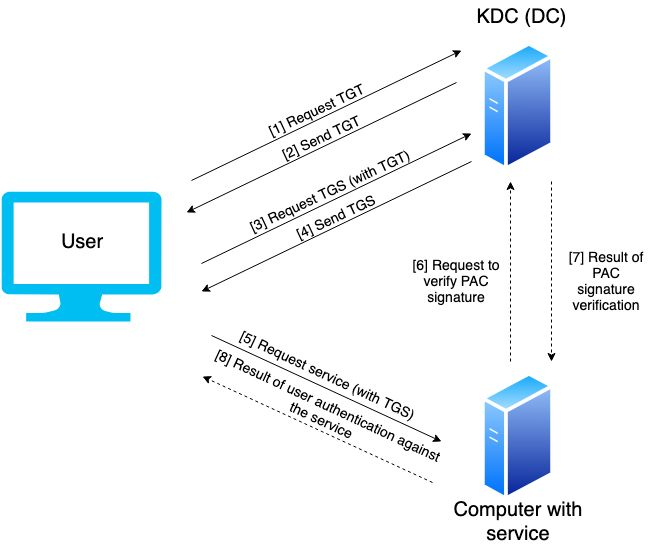
\includegraphics[width=.8\textwidth]{figuras/TGT_TGS_PAC.jpg}
	\caption{Steps for Kerberos authentication}
\end{figure}
\linej
The Golden Ticket attack depends on obtaining the password information of the KRBTGT account to generate a forged TGT. It can provide the attacker with the desired privileges in the AD (like administrator).
\linej
This means TGTs can be generated to access every account within the AD. This forged TGT is known as Golden Ticket.
The Golden Ticket does not depend at all of the administrator password of the AD, which means that changing this password does not invalidate a Golden Ticket in anyway.
\linej
\linej
Because the attack uses a valid TGT is very hard to detect it is a forgery. Once it has been generated the TGT can be used at any time and any amount of times until the time expiration.
Any TGS obtained from a Golden Ticket is no longer a forgery, because is generated from the DC.
\linej
\linej
The password information of the KRBTGT account can be just the hash of the password, which is stored in memory and can be retrieved with enough local privileges in a DC. To generate the Golden Ticket the attacker also needs the domain name and the SID of the domain to which the KRBTGT account belongs, which are trivial to get\cite{stealthbits}.
\linej
Furthermore once the required data is obtained the Golden Ticket can be generated offline using certain programs, like Mimikatz. This means is impossible to detect the creation of the ticket itself if is not done on a computer in the network.
\linej
It follows that this attack can only be detected either during the steps needed to create the TGT (get the hash of the KRBTGT account) or by the use of the TGT.
\linej
\linej
By default Mimikatz sets the forged ticket age to 10 years, which is useful to some attackers because they would need only one attack to compromise the entire network for that time.

\subsection{Exploit methods}
To keep this simple only the basics are explained about the techniques used in the examples for a Golden Ticket attack. Because some of the exploits are similar they are numbered for easier identification. The scripts in the next exploits were used to understand the different ways to perform Golden Ticket attacks and during the tests to try to detect them. Of course there are more ways to generate a Golden Ticket, and some are much more harder to detect, but there is no time to examine them all. Also it is possible to combine several of the next exploits or change some of their steps.
\linej
For example there is a sever-agent version of Mimikatz called Pypykatz\cite{pypykatz_agent}\cite{pypykatz_server} that is very new and should be a bit harder to detect that the exploits showed here. Unfortunately the student could not make it retrieve the KRBTGT hash.
\linej
\linej
These scripts try to automate as much of the process as possible, which is normally done in an interactive way. This automation helps to assure that the results are the same each time and reduces the time for each test. All the tests in this project were executed at least twice. Tests were repeated if there were changes that could affect their results.

\subsubsection{Exploit 1: Local Mimikatz in DC}
This requires local administrator privileges in the DC and also and an already downloaded version of Mimikatz in the DC, which the attacker can easily get after gaining privileges. If this example were to be used as it is it will probably be detected by the antivirus and Windows Defender, but again they can be disabled by a local administrator and there are techniques to avoid being detected by them.
\linej
\lstinputlisting[style=PS,caption=Script to generate and inject a Golden Ticket,captionpos=b]{src/genticket.ps1}
\linej
The script uses Mimikatz to get the needed data to generate the Golden Ticket, saving it to a file for convenience. Then the data is split in variables, each being a piece for generating the forged ticket. The \textit{exit} parameter is to exit the Mimikatz shell after executing the command.
\linej
After injecting the ticket (with the \textit{/ptt} option) the session haves administrator privileges in the AD, so any service in the AD can be used in this powershell session, any command should be allowed. Without the injection option Mimikatz would store the ticket in a file, which can be injected at any time with Mimikatz.
The id 500 is the normal id for the administrator account in the AD.
This script can be executed in multiple ways, for example from a powershell interactive terminal run as an administrator.
\linej
\lstinputlisting[style=txt,caption=Example of the contents of the output file,captionpos=b]{src/output.txt}
\linej
The password hash of the KRBTGT account is retrieved by Mimikatz interacting with the Local Security Authority (LSA) or Local Security Authority Subsystem Service (LSASS), which is run by the lsass.exe process.
\linej
This process is the Windows service responsible for providing single sign-on functionality.
With it users are not required to re-authenticate each time they access resources.
It provides access not only to the authenticated user's credentials, but every set of credentials used by every open session since the last boot\cite{wikipedia_lsass}\cite{dump_ways}.
\linej
Mimikatz exploits this cache of credentials and reports the results to the user in the various forms employed by LSASS\cite{SANS_mimikatz}\cite{pentestlab}.

\subsubsection{Exploit 2: Mimikatz from memory in DC}
This is similar to the previous example but instead of having a downloaded version of Mimikatz (stored in the disk) the program is downloaded directly into the powershell session, so Mimikatz is never stored in disk.
The clear advantage over the previous one is that it should be harder to detect.
\linej
With slight changes this could work in a computer that is not a DC, if the attacker compromised a workstation a domain admin logged onto\cite{dump_ways}.
\linej
\lstinputlisting[style=PS,caption=Script to run Mimikatz only in memory and inject a Golden Ticket,captionpos=b]{src/genticket_mem.ps1}
\linej
The script downloads a version of Mimikatz from Github and creates a powershell object with its contents, that can be invoked at any time in this shell\cite{powersploit}\cite{mimikatz_details}. Then as before it dumps the needed information to generate the Golden Ticket in a file, which is read and parsed to store the interesting parameters into variables.
\linej
Due to difficulties with the last \textit{Mimikatz} command to work with the parameters in the variables a workaround was used. This is writing a new file that has the command with those parameters, and then execute the file.
\linej
\linej
On the one hand it can be harder to detect with obfuscation, renaming and not using such an obvious url.
On the other hand powershell can be monitored for downloading commands, particularly those with objects.

\subsubsection{Exploit 3: Mimikatz with DCSync}
The DCSync is a Mimikatz feature in which a no-DC attempts to impersonate a DC and request account information from a real DC. This technique is less noisy because it does not require direct access to a DC (which are often heavily monitored)\cite{dump_ways}\cite{pentestlab}. To run Mimikatz we still need local administrator privileges in the computer.
\linej
\lstinputlisting[style=PS,caption=Script to run Mimikatz with DCSync,captionpos=b]{src/genticket_dcsync_mimikatz.ps1}
%some times the dcsync Mimikatz command does not work and needs to restart the no DC computer
\linej
This follows the same structure as the previous cases, but this time with the dcsync option.
The disadvantage in this case is that there needs to be a connection to a running DC that is not being monitored for the requests Mimikatz sends. There are open source tools available for this kind of monitoring\cite{dcsync_monitor} and it can also be detected by monitoring the network\cite{dcsync_monitor_network}.

\subsubsection{Exploit 4: DCSync with Kiwi}
In this case the access to the no-DC computer in the targeted network is done through Metasploit\cite{metasploit} and its own version of Mimikatz called Kiwi\cite{pentestlab}. The Kali virtual machine is for running Metasploit outside the AD, but a Windows machine running in the AD could have been used as well.
\linej
We need to know the password of the account we want to access remotely and the targeted computer needs to have a SMB share.
In this case the variable \textit{SMBPass} stores the password, which is \textit{Passw0rd}.
\linej
\lstinputlisting[style=ruby,caption=Part 1 of the remote DCSync exploit automation,captionpos=b]{src/metasploit_p1_kiwi.rc}
\linej
This runs a remote process, exploiting the SMB capabilities to run commands to spawn a Meterpreter shell\cite{meterpreter} with administrator privileges. There is a chance that the \textit{run} command fails to provide a Meterpreter shell at this stage, but trying again always ends working because the session is not getting created even though the exploit is working.
\linej
\linej
Now we are in a Meterpreter shell, which we can use to get the exact privileges we need for the next part. This is because even though we have administrator privileges there are different kinds of administrator privileges on Microsoft systems.
\begin{figure}[H]
	\centering
	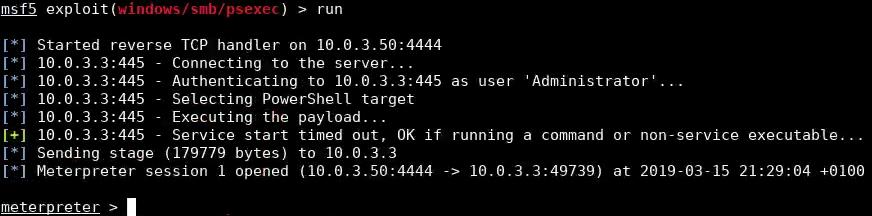
\includegraphics[width=\textwidth]{figuras/meterpreter.png}
	\caption{Meterpreter shell running}
\end{figure}

To do this we look for a session running administrator privileges in the AD. In this case the targeted machine had a powershell session running as administrator, to which we migrate.
\linej
\begin{figure}[H]
	\centering
	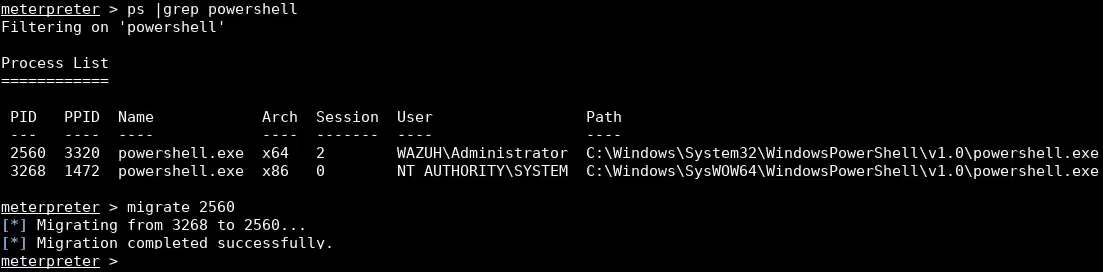
\includegraphics[width=\textwidth]{figuras/migrate.png}
	\caption{Migration to a powershell session as AD administrator}
\end{figure}

Now we are ready to run the real exploit. This loads the Metasploit version of Mimikatz (Kiwi) in the Meterpreter shell, allowing the attacker to use Kiwi commands.
The command in this case retrieves the information of the KRBTGT account needed to generate the Golden Ticket.
\linej
In this case the generation of the ticket is not using the data in an automated way, because there was no real need since is the same every time and the time needed to do this with Ruby felt like a waste. In this case the ticket is saved to the \textit{/tmp/golden.tck} file in the Kali machine.
\linej
\lstinputlisting[style=ruby,caption=Part 2 of the remote DCSync exploit automation,captionpos=b]{src/metasploit_p2_kiwi.rc}
\begin{figure}[H]
	\centering
	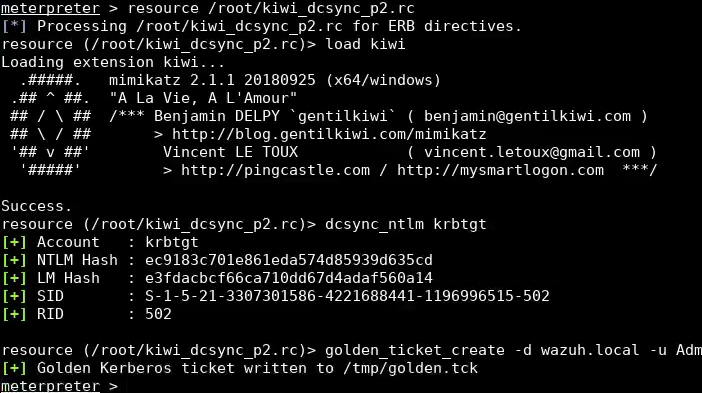
\includegraphics[width=\textwidth]{figuras/kiwi_p2.png}
	\caption{Retrieval of KRBTGT data and generation of the Golden Ticket with Kiwi}
\end{figure}
The obvious downside of this method for the attacker is that Metasploit is very widely used and known, therefore there could be security monitoring for it\cite{detect_metasploit_traffic}. But again the attacker is using a technique that does not need to control a DC and does not need to store anything in the disk of the targeted system, making it much harder to detect in that regard.
\linej
\linej
Of course there is no real need to use Metasploit to get a remote shell to run Mimikatz. The attacker could use ssh, run remote commands with \textit{psexec} or use the Windows Remote Shell. But some of these need to be enabled and they would not be much different of the previous examples.

\subsubsection{Exploit 5: Hashdump with Meterpreter}
Using a reverse TCP exploit the attacker access the targeted DC with a Meterpreter shell. This is similar to the previous case but using the Meterpreter command \textit{hashdump} instead of the DCSync retrieval of Kiwi\cite{pentestlab}. This stills uses Kiwi to generate the Golden Ticket.
\linej
\lstinputlisting[style=ruby,caption=Part 1 of the remote Hashdump exploit automation,captionpos=b]{src/metasploit_p1_hashdump.rc}
\linej
Again there is a migration to an administrator account of the AD. In this case another command to get the SID of the network would be needed if we did not know it already, for example a simple \textit{whoami /user} would suffice.
\linej
\lstinputlisting[style=ruby,caption=Part 2 of the remote Hashdump exploit automation,captionpos=b]{src/metasploit_p2_hashdump.rc}
\begin{figure}[H]
	\centering
	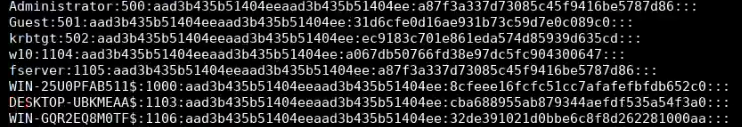
\includegraphics[width=\textwidth]{figuras/hashdump.png}
	\caption{Retrieval of KRBTGT data with hashdump}
\end{figure}
As before it is expected of the DCs to be more monitored. This means that the DCSync version is more interesting to an attacker because it has the same difficulty and benefits at a lower risk.

\subsection{Detection purely with signatures}
Searching for suspicious strings can be used to trigger alerts with Wazuh.
Signature matching of data coming from Windows events and default logs from Windows systems is not much different from what any antivirus do. It follows that it would be as easy to evade as them. For example with substitution of suspicious strings from the source code and recompilation\cite{understanding_powersploit_mimikatz}.
\linej
\linej
This does not mean that signature matching is totally worthless, but that it is not something to focus on. In this project relying in signatures was avoided as much as possible.
Useful signatures to match not only amount to third-party tools. It is easy to monitor extensions, directories, certain files, command line options, usernames, etc.
\linej
Obviously matching some signatures is more valuable than matching others. For example finding \textit{Mimikatz.exe} is easier to implement and less valuable than \textit{krbtgt}, \textit{lsadump}, \textit{kerberos::} or \textit{privilege::}.
\linej
\linej
As we know the techniques to detect or avoid detection evolve with each other over time.
Any way we manage to detect programs like Mimikatz may be overcome in the future.
\linej
That does not mean that detection techniques are bound to fail or that there is no point to them.
Many attackers know how hard it can be to overcome detection techniques.
\linej
It is also important to remember these scenarios are continuously changing, with new techniques to avoid detection and the creation of new tools.

\subsection{Detection purely with Windows events}
In theory we can identify certain attacks only with the security events of Windows. There are multiple websites in which this attack has been analyzed and its events identified\cite{events_1}\cite{detection_events}.
\linej
Unfortunately the events recorded did not always probe to be the same as the cited sources (probably because it was tested on the new Windows Server version, 2019).
In most cases their frequency is not enough to be distinguished of the regular activity, even when using a lab environment without work load.
This could probably be improved if these events had more information (particularly those as critical as Kerberos'), but they are very short and generic.
\linej
\linej
Wazuh provides access to Windows events by default, due to the rules and decoders of its ruleset\cite{wazuh_ossec_ruleset}, the user only needs to define rules to specify what and how he wants to monitor.
\linej
We can enable additional logging with the Advanced Audit Policy Configuration. For example for auditing kernel objects, more Kerberos logging, changes in settings or account events.
\linej
\linej
The student tried to analyze the security events to find patterns in the previous exploits, by recording all the data received by Wazuh in during their execution. This was done just by looking the current line of the log, executing the exploit and copying the log from there to a new file.
\linej
The obvious problem of this method is that it results in logs with tens to hundreds of lines filled with a not very easy to read format. The workaround used was to parse the logs with custom AWK scripts\cite{memoria_github}, removing fields to make the logs more readable and counting each of the events in them.
\linej
\linej
The idea of finding a relationship between certain windows events and this attack was abandoned because:
\begin{itemize}
	\item It was not providing any new results.
	\item It was too time consuming.
	\item It can be accomplished using Sysmon\cite{sysmon}\cite{sysmon_event_7_mimikatz}.
	\item Also it was concerning the amount of noise this method has, even though in a laboratory without real system load, to tell apart an intrusion from a totally healthy system.
\end{itemize}
\linej
The real useful addition to the Windows builtin events is having Sysmon\cite{sysmon} in each of the monitored Windows computers. They can be combined to identify attackers better\cite{detection_events}.
\linej
With Sysmon we can have reports of events [1-21] and 255, which in some cases provide very precise and useful information of the system. For example we can configure Sysmon to log data about process with a certain processes, like: \textit{powershell}, \textit{Mimikatz}, any \textit{.ps1} or any \textit{.exe}.
Sysmon can monitor each of the events either by whitelisting or blacklisting by default or both. We can also combine it with rules from Wazuh, using Sysmon to increase the report capabilities and Wazuh to filter them.
\linej
\linej
Also is important to note that Sysmon can be a bit tricky to balance the configuration to get as much suspicious events as possible, while not reporting so much it affects the performance of the network. This is responsibility of the administrators of the network, who also have to tune the configuration to their custom needs.
There are public configs for Sysmon that attempt to provide a good insight of the system while not logging too much data\cite{sysmon_config}.

\subsection{Detection of Mimikatz}
Mimikatz is the tool of choice for this kind of attack for most attackers because it is very effective, easy to use and has multiple ways to be used in different attacks\cite{mimikatz_github}\cite{mimikatz_details}. This is a double edge sword for Mimikatz because it has become one of the programs to look for in antimalware detection programs. In this case we assume these programs have not detected Mimikatz and is up to Wazuh to do it. It is interesting to note that the author of Mimikatz provides ways to detect it, like the YARA rules he maintains\cite{mimikatz_github} or BusyLights\cite{understanding_powersploit_mimikatz}.
\linej
\linej
Detecting Mimikatz is not a sign of a Golden Ticket attack (unless is clear in the way it is used), but still it is a big and dangerous threat to the system and worth checking out.
\linej
Unfortunately as seen in the exploits before there are multiple ways to execute Mimikatz, in an attempt not to be discovered by known techniques.
\linej
\linej
Each time a Mimikatz shell spawns certain DLLs are loaded. The technique to identify a succession of events in a short time as another event is called grouping.
Grouping is a very effective technique, but it may require a lot of work to identify its components. In some cases the attack may not produce enough noise or it may not be possible to tell it apart from the normal events of the system\cite{sysmon}\cite{sysmon_event_7_mimikatz}.
\linej
Fortunately Mimikatz needs a fair amount of DLLs to work and some of them are not very usual. This makes the execution of Mimikatz noticeable.
\linej
\linej
 The load of a DLL can be detected by the event 7 of Sysmon and the grouping can be identified with Wazuh rules. It also can be detected by the event 10 of Sysmon, for inter-process access, but a greater cost of bandwidth.
For this task is better to configure Sysmon to monitor these 5 images, to avoid logging too much:
\linej
\lstinputlisting[style=xml,caption=Sysmon monitoring with event 7 for certain DLLs,captionpos=b]{src/sysmon_event_7.xml}
\linej
On the manager side the next rules are needed:
\linej
\lstinputlisting[style=xml,caption=Rules for suspecting a Mimikatz execution as a group of events,captionpos=b]{src/rules_event_7_mimikatz_alternative.xml}
The \textit{sysmon\_event7} means that another rule has marked the log as a Sysmon event of type 7.
\linej
The \textit{same\_field} option means that every one of the matches must have the same value in the designed field, which in this case means that these events come from the same computer.
\linej
The \textit{frequency} option means that the rule has to be matched that number of times to trigger. Is set to 2 because is the minimum value possible.
\linej
\linej
Normally each of the suspicious DLLs would have its own rule, but it would not always identify Mimikatz because the frequency has to be at least 2. Therefore rules \textit{300301} and \textit{300302} identify 2 and 3 DLLs each (using a logical OR), making it possible to trigger the grouping rule.
The last rule identifies the use of the DLLs in a 10 seconds gap as the execution of Mimikatz. This detection could be evaded by adding time between the load of the DLLs in the source code.
\linej
\linej
The problem of these less precise rules is that it is possible to have false positives. None were seen during this project for this case.
\linej
Unfortunately due to the way OSSEC matches rules there is no way to have an hierarchy of rules to trigger a precise grouping rule or the other one.
\linej
\linej
Detecting the use of every variant of Mimikatz is virtually impossible, not only because their sheer number due to its popularity but because anyone can compile their own. Therefore the logical way to detect Mimikatz would be to detect the basic step for every version: the interaction with the LSASS and process injection. More can be read on page \pageref{detect_lsass}.

\begin{table}[H]
	\centering
	\begin{tabular}{|l|l|l|}
		\hline
		\rowcolor{gray!30}
		Exploit & Detected \\ \hline
		1: Local Mimikatz in DC& \RYES\\ \hline
		2: Mimikatz from memory in DC& \RYES\\ \hline
		3: Mimikatz with DCSync& \RYES\\ \hline
		4: DCSync with Kiwi& \RYES\\ \hline
		5: Hashdump with Meterpreter& \RYES\\ \hline
	\end{tabular}
	\caption{Exploit detection by grouping events}
\end{table}
This method detects the use of Mimikatz in all the ways implemented in this project.
The hashdump exploit is detected because Kiwi is used in the session in that machine to generate the Golden Ticket. A real attacker probably would generate the ticket outside of the network, avoiding being detected by this technique.

\subsection{Detection of the use of the TGT with klist} \label{klist_detection}
We can not always detect when a forged TGT is generated, but the attacker still needs to use it to gain access to the active directory domain with the privileges set in the ticket. The first choice for this task would be to monitor the Kerberos log searching for unusual patterns, but it proved to be more hard than it should, so instead a scan the cache of Kerberos tickets every few minutes was implemented.
\linej
The program to examine the contents of the cache is \textbf{klist}.
\linej
\linej
In order to do this we need to enable the execution of Wazuh's remote commands in the Windows agent and set the properties of the command in the manager in \textit{/var/ossec/etc/shared/default/agent.conf}\cite{wazuh_remote_command}:
\linej
\begin{lstlisting}[style=xml]
<agent_config os="Windows">
	<wodle name="command">
		<disabled>no</disabled>
		<tag>remoteklist</tag>
		<command>powershell C:\\Users\\Public\\Documents\\klist.ps1</command>
		<interval>5m</interval>
		<ignore_output>no</ignore_output>
		<run_on_start>yes</run_on_start>
		<timeout>0</timeout>
		<skip_verification>yes</skip_verification>
	</wodle>
</agent_config>
\end{lstlisting}
\linej
In this case the command is a script to get all the tickets of all the sessions with klist, compare the ticket value for the field \textit{TicketExpireHours} with the value of \textit{MaxTicketAge} of the Group Policy (putting the difference in a new field) and parse the output to JSON. Having the output in JSON makes it a bit easier to read from the logs (which is useful to fix any mistake in the script) and removes the need of a decoder in the manager.
The idea came from a very different klist script that only works interactively and reports in plain text\cite{klist_script_idea}.
\linej
This script needs to be run in every member of the network to guarantee detection for every user.
\linej
Doing this with only powershell assures it will work in any Windows system without external programs. The downside of this parsing and my limited knowledge of powershell is that the script is a bit bulky and the dependency on the format of the output of klist.
\linej
\lstinputlisting[style=PS,caption=Script to scan and parse to JSON the tickets in the cache,captionpos=b]{src/klist.ps1}
\lstinputlisting[style=PS,caption=Way to get the MaxTicketAge from the Group Policy,captionpos=b]{src/report.ps1}
\linej
Unfortunately that way to get the \textit{MaxTicketAge} from the Group Policy in the last script does not work by default with remote commands because Windows remote commands only allow certain types of commands.
In any case the \textit{MaxTicketAge} value is not normally changed and it requires AD administrator privileges to do it, so due to the time constrains of the project this automation was abandoned. There are other ways to get the \textit{MaxTicketAge} value, but as mentioned is not something to spend time on.
\linej
\linej
Next there is an example of the difference between the normal output of klist and the string stored in an alert in the manager.

\begin{figure}[H]
	\centering
	\includegraphics[width=.9\textwidth]{figuras/klist_normal.png}
	\caption{Klist listing tickets for a certain session}
\end{figure}
\begin{figure}[H]
	\centering
	\makebox[\textwidth][c]{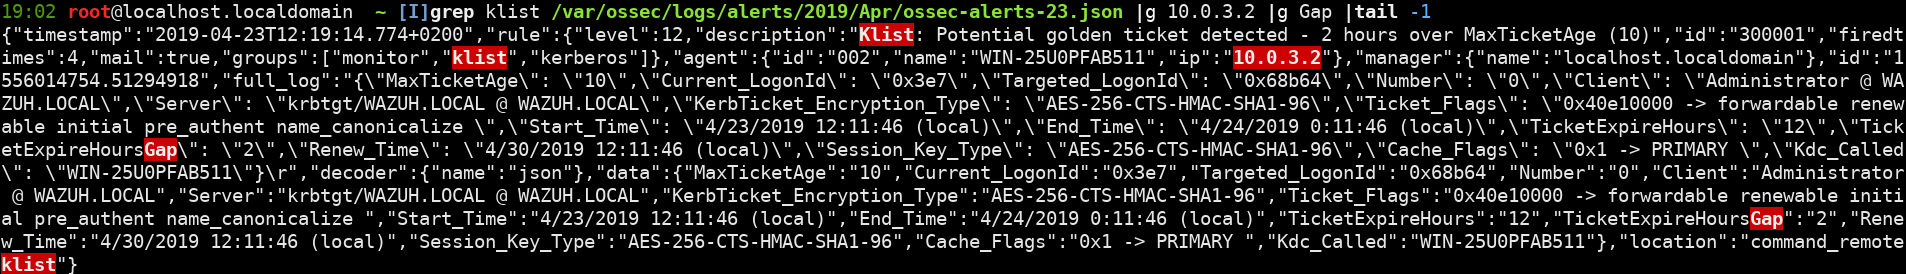
\includegraphics[width=1.2\textwidth]{figuras/klist_alert.png}}
	\caption{Latest alert of the klist monitoring in the manager}
\end{figure}
\linej
The time difference mentioned before is a very easy way to detect a forged ticket. With a simple subtraction in the powershell script only a rule that makes a number comparison in the manager is needed to launch the alert.
\linej
\lstinputlisting[style=xml,caption=Rules to detect a suspicious expiration age from the report of the klist script,captionpos=b]{src/rules_klist.xml}
\linej
The purpose of the first rule is to identify any log in JSON with \textit{MaxTicketAge} and \textit{TicketExpireHours} fields. The second rule is used to examine the contents of the \textit{TicketExpireHoursGap} field of the logs that the first rule has identified. If the value of the \textit{TicketExpireHoursGap} field starts with a digit different than 0 then it means that \textit{MaxTicketAge} $>$ \textit{TicketExpireHours}, therefore the expiration age is greater that it should, triggering an alert.
Additionally it can only trigger once each 600 seconds, to avoid flooding of alerts.
\linej
\linej
This attack is often used because it may grant the highest privileges in the domain, is hard to detect and is very persistent because it does not care for the password changes in the active directory. That is why is very attractive for domains in which the attacker may decide to come back later, maybe even years later. That means is very unlikely for a forged ticket to not have a very big expiration age, because is one of its most appealing benefits; but again it would be possible to an attacker to keep generating forged tickets with a valid expiration age forever, at a greater risk of being detected in other ways.
\linej
\linej
The testing of the script was satisfactory, the cases that inject a TGT were detected and there were no false positives:
\begin{table}[H]
	\centering
	\begin{tabular}{|l|l|l|}
		\hline
		\rowcolor{gray!30}
		Exploit & Detected & As expected \\ \hline
		1: Local Mimikatz in DC& \RYES& \RYES\\ \hline
		2: Mimikatz from memory in DC& \RYES& \RYES\\ \hline
		3: Mimikatz with DCSync& \RYES& \RYES\\ \hline
		4: DCSync with Kiwi& \RNO& \RYES\\ \hline
		5: Hashdump with Meterpreter& \RNO& \RYES\\ \hline
	\end{tabular}
	\caption{Exploit detection by the klist script}
\end{table}
Of course if we chose to store the ticket in a file we could inject it in other moment or computer, but then it could be detected by this method.
\linej
\linej
Additionally there could be monitoring for unusual usernames, because is possible to get a TGT with administrator privileges with non existent username to avoid the monitoring that administrator accounts are often under.
\linej
\linej
It can be worth checking if the attacker is using klist to clean the cache of injected tickets, to cover any tracks. This can be easily accomplished monitoring the execution of klist with the event 1 of Sysmon:
\begin{lstlisting}[style=xml]
<ProcessCreate onmatch="include">
	<Image condition="contains">klist</Image>
</ProcessCreate>
\end{lstlisting}
\linej
And checking with Wazuh if the option \textit{purge} was used:
\lstinputlisting[style=xml]{src/rules_klist_purge.xml}

\subsection{Silver Ticket}
A Silver Ticket is very similar to a Golden Ticket, is a forged TGS instead of TGT. Therefore a Silver Ticket only grants access to a service in a computer. Is important to note that some services need the privileges of more services, therefore more than a Silver Ticket may be needed.
\linej
Steps 1 and 2 of a normal Kerberos authentication exchange are not needed (figure \ref{kerberos_exchange}) because they are only to get a TGT. Without a TGT a TGS can not be requested from the DC, so steps 2 and 3 are also not a part of the Silver Ticket attack.
\linej
There is no need to connect to a DC, only a connection to the computer hosting the service is needed (steps [5-8]). Unless PAC validation is required, the service accepts all data in the TGS ticket.
\linej
The TGS is ciphered with the password hash of the account running the service, making changes of the password an effective mitigation against Silver Tickets.
To extract this data from memory the attacker has to have local administrator privileges\cite{events_1}\cite{silver_ticket}.
\linej
\linej
To extract the data the attacker would need to run Mimikatz with:
\begin{lstlisting}[style=PS,numbers=none]
"privilege::debug" "sekurlsa::logonpasswords" exit
\end{lstlisting}
\linej
For example in the next scenario:
\begin{itemize}
	\item The user to impersonate is the AD Administrator.
	\item The computer is is \textit{WIN-GQR2EQ8M0TF}.
	\item The domain is \textit{wazuh.local}.
	\item The domain is identified as \textit{S-1-5-21-3307301586-4221688441-1196996515}.
	\item The attacker wants access to the \textit{HOST} service.
	\item The password hash of the account is \textit{68fbd238f574f7685beed96a2db15004}.
\end{itemize}
The Mimikatz command would be:
\begin{lstlisting}[style=PS,numbers=none]
"kerberos::golden /admin:Administrator /id:500 /sid:S-1-5-21-3307301586-4221688441-1196996515 /domain:wazuh.local /target:WIN-GQR2EQ8M0TF.wazuh.local /rc4:68fbd238f574f7685beed96a2db15004 /service:HOST /ptt" exit
\end{lstlisting}
Allowing the attacker to access the \textit{HOST} service on that computer with AD Administrator privileges.
\linej
\linej
Silver Tickets get registered in the Kerberos' cache in the same way as the Golden Tickets, so they can be detected with the klist script. The execution of Mimikatz can be detected with grouping just as before.

\subsection{Mitigation}
These exploits take advantage of the inherent weaknesses of Kerberos, so there is no way to prevent them. Nevertheless, Microsoft provides a public guide explaining how to mitigate this kind of attacks\cite{microsoft_mitigation}.
The easiest way to mitigate this attack is to change the password of the KRBTGT account to invalidate any existing Golden Ticket, which has to be done twice (make sure the domain converges before doing the second password change\cite{hood}), but it also invalidates existing proper TGTs.
\linej
The recommendation from Microsoft is to regularly reset the password\cite{tarlogic_comprehension}\cite{adsecurity_483}, which can be done with their official script\cite{reset_script}. This could be also triggered by alerts that we are confident detect Golden Tickets, but as mentioned this could affect other functionality and so the decision is for the network administrators to make. Any TGT that is not valid produces an error in a TGS request, which can be used for exposing an attacker\cite{scom_GT}.
\linej
\linej
Also there are other measures like:
\begin{itemize}
	\item Have administrative passwords longer than 25 characters to avoid brute force cracking and make them unique for each system.
	\item Enforce a least privilege model.
	\item Minimize the quantity of administrative accounts.
	\item Isolate DCs: Use DCs only as servers, never work stations of any kind.
	\item Isolate administrator accounts: Use administrator accounts only for administrator duties.
	\item Isolate AD accounts: Create tiered groups with very granular permissions on the domain and create Access Control List permissions on the Organization Units of the AD\cite{AD_tier}.
	\item Use Read Only Domain Controllers (RODCs): keep Read Write DCs segregated using network segregation and AD sites to force users to logon to RODCs, making breach detection easier. RODCs don't have any real user hashes (nor the hash of the KRBTGT account)\cite{hood}\cite{reset_RODC}.
	\item Use honeypots: With populated the LSASS cache with false credentials\cite{SANS_mimikatz}\cite{honeyhashes} or with decoy AD objects\cite{decoy_AD}. And then monitor the logs for attempts to use them. This can lead to detect attackers or to find vulnerabilities in the network.
	\item Disable storage of clear text passwords in LSASS memory to limit the information provided by Mimikatz\cite{SANS_mimikatz}.
	\item Run LSASS in protected mode (from Windows 8.1): calls to LSASS are only allowed by other protected-mode processes\cite{SANS_mimikatz}\cite{understanding_powersploit_mimikatz}.
	\item Use choke points: Create a choke point for access to your DCs, adding another layer of protection. Create a Terminal Server that can only talk to the DCs. Configure the DCs to only accept administrative connections from that Terminal Server\cite{choke}.
\end{itemize}
\linej
We could go on with more detail and increasing the mitigation\cite{AD_defense}, but is not the objective of this project.

\subsection{Conclusion}
We have seen how the data to generate Golden Tickets can be obtained in different ways and the difficulties for both the attacker and the defender roles.
\linej
\linej
Relying on the klist detection means there is no real need to detect each of the different ways to generate the Golden Ticket because it may be impossible depending on the circumstances. More importantly the attacker still needs to present it to a DC to get the TGSs, to get any benefit from the Golden Ticket.
\linej
Detecting certain Sysmon events in a close time gap can guarantee the detection of Mimikatz, therefore detecting one of the most used ways to gather this data. Detecting certain signatures for running commands, reads and accesses are a worthy way to detect the creation of a Golden Ticket, without spending much resources.
\linej
These are good examples of how detecting common steps to multiple exploits is one of the strong points of an HIDS.
\linej
\linej
Another way of detection is to use YARA to look for certain patterns in memory, just like we can search for strings in the events. In the case of events the data comes from the program, which is easy to modify with multiple techniques like substitution or obfuscation. The patterns in memory are much more harder to change because it involves changing the logic of the program. That means most attackers would just take the risk to be detected by this kind of technique.
\linej
YARA is very interesting for this kind of project, but it belongs to the Virustotal pack of malware detection tools and so it could be used with Wazuh with a Virustotal API key. The free version only allows a few queries and the option of getting a premium key was not considered. There has been for months an open issue in the Github page of Wazuh for integrating it with YARA (as other IDSs have done before), which has recently evolved to an issue to integrate YARA into Wazuh as a module\cite{yara_module}.
%Unfortunately this was not done before this part of the project as completed, so there was no time left to investigate more on it.
%TODO revisar estado issue en el futuro


\section{More about the extraction of credentials}
In the previous section the extraction of credentials was explained to understand the details surrounding a Golden Ticket attack. This includes extracting password hashes from the memory of the LSASS process with Mimikatz or Hashdump. But there are more ways of extraction that are used against AD network now a days.
\linej
Once credentials have been retrieved an attacker has more options, like generating a Golden Ticket.
The key points of access are the \textit{NTDS.DIT} file that is stored in disk and the running process \textit{lsass.exe}.

\subsection{Exploit methods}
Because the database file of the AD accounts is locked from copying and reading, only Windows tools are allowed to. These tools are \cite{dump_ways}:
\begin{itemize}
	\item Reg: Allows to change or save registry hives, including those that contain credentials.
	\item Ntdsutil: Provides management of this database, including creation of backups.
	\item WMIC: Commands for the Windows Management Instrumentation. They allow all kinds of remote management, including copy of files using Shadow Copy.
\end{itemize}
Another way to extract these credentials is to dump them from memory using third party tools and scripts. This is saving part of the data of a process running in the system\cite{dump_ways}.
There are multiple tools available for this, but in this project only these were used: Mimikatz, Hashdump, ProcDump, pd, Minidump and NinjaCopy.
\linej
Some of these tools have the option to retrieve the password or hashes history, meaning that the attacker could gain valuable insight on the password policy of the target.
\linej
\linej
There was no effort to automate these exploits because they are too simple.
All the extraction programs were executed with local administrator privileges in a DC.

\subsubsection{Exploit 6: Retrieval of NTDS.DIT with ntdsutil}
Another way to get the desired information is to copy the database of the AD Domain Services (the NTDS.DIT file) and conduct an offline password audit of the domain. This means once we have this data we can use a wide selection of tools to crack it\cite{ntdsdit_tools}\cite{extracting_ntds}\cite{ntds_powershell}.
\linej
\linej
The attacker has to open a shell as administrator in a DC to create the backup. Multiple commands or an one-liner can be used:
\begin{lstlisting}[style=PS,frame=none]
ntdsutil "activate instance ntds" ifm "create full C:\temp\ntdsutil" quit quit
\end{lstlisting}
\linej
This command creates a ntdsutil shell and activates the instance to later create a backup in a temporary directory (inside the ifm subshell).
\begin{figure}[H]
	\centering
	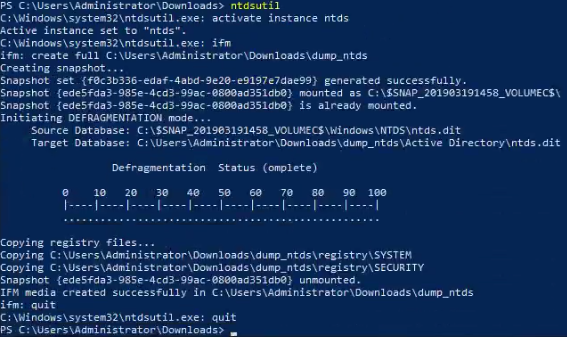
\includegraphics[width=\textwidth]{figuras/ntdsutil.png}
	\caption{Backing up the database of the AD using the ntdsutil shell}
\end{figure}
There are other ways to use ntdsutil in ways harder to detect\cite{more_dumps}, but this is enough for gathering events for analysis.
\linej
\linej
The creation of processes related to ntds can be reported by Sysmon:
\begin{lstlisting}[style=xml]
<ProcessCreate onmatch="include">
	<Image condition="contains">ntdsutil.exe</Image>
</ProcessCreate>
\end{lstlisting}
\linej
And alerts set with Wazuh:
\lstinputlisting[style=xml]{src/rules_ntds.xml}
\linej
The first rule is the parent, it filters windows events with the \textit{ntds} string.
\linej
The second rule detects the ntdsutil executable. This signature is more useful than normal because it is a builtin tool. The third matches \textit{ntds} for the command line, which is not really reliable.
\linej
The rest are for detecting suspicious database events from Windows events. These database events assure the detection of ntdsutil even if it were to be executed without using known signatures.
\linej
\linej
There is also the remote version of Reg: WinReg. But there was no time to investigate on it. Is likely that it can be detected with network monitoring, as other remote tools.

\subsubsection{Exploit 7: Storing registry hives with Reg}
These commands produce the different save files, each of a different group of credentials, that can be later extracted offline with certain tools\cite{more_dumps}:
\begin{lstlisting}[style=PS]
reg.exe save hklm\sam c:\temp\sam.save
reg.exe save hklm\security c:\temp\security.save
reg.exe save hklm\system c:\temp\system.save
\end{lstlisting}
\linej
Reg is not detected as malware because it is a builtin tool in Windows. With Sysmon we can report the execution of Reg with the event 1, reporting the creation of a process:
\begin{lstlisting}[style=xml]
<ProcessCreate onmatch="include">
	<Image condition="contains">reg.exe</Image>
</ProcessCreate>
\end{lstlisting}
\linej
And Wazuh to trigger an alert:
\lstinputlisting[style=xml]{src/rules_reg.xml}
\linej
The parent rule matches the creation of Reg from the report of Sysmon.
\linej
The second rule detects the \textit{save} string in the reg command.
\linej
The rest of the rules detect the registry strings for credentials.
\linej
\linej
This also could be detected using the event 7, but it would interfere with grouping detection. Of course it is possible that these rules do not cover all the extraction uses of Reg. Is worth noting that this is a signature base detection, therefore it could be overcome with certain third-party programs.
\linej
\linej
Additionally a grouping detection for the DLLs Reg uses was tested. It detected Reg events every time without relying on the \textit{reg.exe} signature, but there were false positives, particularly during boot.

\subsubsection{Exploit 8: Dump of LSASS with ProcDump}
ProcDump\cite{procdump} is a command-line utility whose primary purpose is monitoring an application for CPU spikes and generating crash dumps during a spike. This program can be used to create a dump file of the running \textit{lsass.exe} process:
\begin{lstlisting}[style=PS,numbers=none]
C:\Users\Administrator\Downloads\procdump.exe -accepteula -64 -ma lsass.exe c:\temp\lsass.dmp
\end{lstlisting}
\linej
The dumped file can be used to extract the credentials by other programs, like Mimikatz\cite{more_dumps}. This is also true for the next exploits.

\subsubsection{Exploit 9: Dump of LSASS with pd}
ProcessDumper, also known as pd\cite{pd}, is another program to dump the \textit{lsass.exe} contents. For example if the id of the process is 552:
\begin{lstlisting}[style=PS,numbers=none]
C:\Users\Administrator\Downloads\pd.exe -p 552 > c:\temp\lsass.dump
\end{lstlisting}

\subsubsection{Exploit 10: Dump of LSASS with Minidump}
Minidump is a script from the PowerSploit Post-Explotation Framework\cite{powersploit}. It can be combined with the \textit{Get-Process} builtin to dump the process into a file:
\begin{lstlisting}[style=PS]
Import-Module c:\users\administrator\downloads\PowerSploit-master\Exfiltration\Out-Minidump.ps1
Get-Process lsass | Out-Minidump -DumpFilePath c:\temp
\end{lstlisting}

\subsubsection{Exploit 11: Dump of LSASS with NinjaCopy}
%%fixes needed
%%	%https://github.com/PowerShellMafia/PowerSploit/commit/bd6fe64316afe293d6b4cdf095ed3cfb64b6ab25
%%	%https://github.com/PowerShellMafia/PowerSploit/issues/293
Another PowerSploit module that can be used to dump LSASS into a file is \textit{NinjaCopy}:
\begin{lstlisting}[style=PS]
Import-Module C:\Users\Administrator\Downloads\PowerSploit-master\Exfiltration\Invoke-NinjaCopy.ps1
Invoke-NinjaCopy -Path "c:\windows\ntds\ntds.dit"  -LocalDestination "c:\temp\ntds.dit"
\end{lstlisting}
\linej
Or to copy the NTDS.DIT of the DC in this laboratory to a no-DC computer:
\begin{lstlisting}[style=PS]
Import-Module C:\Users\Administrator\Downloads\PowerSploit-master\Exfiltration\Invoke-NinjaCopy.ps1
Invoke-NinjaCopy -Path "c:\windows\ntds\ntds.dit"  -LocalDestination "c:\temp\ntds.dit" -ComputerName "WIN-25U0PFAB511"
\end{lstlisting}
\linej
This module allows any file, even if it is locked, to be copied without starting suspicious services or injecting in to processes. This is because it can copy \textbf{any file} from a NTFS volume, by opening a read handle to the entire volume, therefore bypassing the following protections\cite{dump_ways}:
\begin{itemize}
	\item Files which are opened by a process and cannot be opened by other processes, such as the NTDS.dit file or SYSTEM registry hives. This is known as locking the file.
	\item Flags set on a file to alert when the file is opened. Windows can not set a flag because NinjaCopy does not use a Win32 API to open the file.
\end{itemize}
\linej
The code to parse NTFS is loaded with a reflective DLL, making it harder to detect because it does not use the Windows loader nor a DLL file.
\linej
The direct read of the device can be reported with the event 9 of Sysmon, but event 1 can be useful to make sure in the remote case. This needs to be in the configuration file of Sysmon in the DC:
\begin{lstlisting}[style=xml]
<ProcessCreate onmatch="include">
	<Image condition="contains">wsmprovhost.exe</Image>
</ProcessCreate>
<RawAccessRead onmatch="include">
	<Image condition="contains">powershell.exe</Image>
	<Image condition="contains">wsmprovhost.exe</Image>
</RawAccessRead>
\end{lstlisting}
\linej
\lstinputlisting[style=xml,caption=Rules for detecting NinjaCopy,captionpos=b]{src/rules_ninjacopy.xml}
\linej
The local case only generates an event of type 9 and its only signatures are \textit{powershell} and \textit{Device{\textbackslash}HarddiskVolume}. It does not even record the name of the file because the handle is for the volume. This can not really guarantee this event comes from the execution of NinjaCopy, but until now has always worked and never reported a false positive. This rule could be much more useful if the NTDS.DIT file were in a different volume than normal.
\linej
\linej
The remote case is much more easier to detect. In the tests it spawned at least 4 events of each type in about 12 seconds, all from the DC.
The bigger the NTDS.DIT file and the slower the connection the more events are produced.
\linej
The remote command is executed by the \textit{wsmprovhost} program, which stands for Windows Remote Powershell Session.
The contents of the logs of the event type 1 are easy to distinguish from normal, due to the constant value of the \textit{commandLine} and \textit{parentCommandLine} fields.
\linej
The second and third rules detect the events of type 1 and 9 for the remote execution, and the last rule is a grouping rule of these two. This assures there are no false positives, but the second rule matches the exploit so well that it could be left out and probably would never cause false positives.
\linej
If the remote command is executed from DC and set to copy from the same computer it still triggers the remote alert.
\linej
\linej
Grouping the DLLs loaded by the \textit{Import-Module} command probed to be effective. As with Mimikatz, this loads the DLLs needed for NinjaCopy to work, which can be registered by the event 7 of Sysmon:
\lstinputlisting[style=xml]{src/sysmon_event_7_ninjacopy_import.xml}
\linej
These 8 DLLs are detected by 4 rules to reach the minimum frequency:
\lstinputlisting[style=xml]{src/rules_ninjacopy_import.xml}
\linej
No false positives were found, but they may appear in a real environment. This technique depends too much on the time frame and can be avoided changing the code. It works with both local and remote cases the same.
%\linej
%\linej
%The next detection attempt was to use a grouping technique for the DLLs the program uses during the copy process. All of them were monitored with the event 7 of Sysmon. The most frecuent were: advapi32, kernel32, kernelbase, msvcrt and ntdll.
%\linej
%These DLLs are used very often in any healthy system. The script did not increase their use too much, therefore false positives were produced during normal execution, discarding this method of detection.

\subsection{Detection of process accessing LSASS} \label{detect_lsass}
The event 10 of Sysmon reports when a process access another process, possibly detecting hacking tools that read the memory contents of processes\cite{sysmon}.
This event can be used to detect LSASS dumps, at least in some cases\cite{sysmon_event_10_lsass}.
\linej
The downside is it can generate significant amounts of logging, therefore it was configured to log only the LSASS process and exclude the instances from the OSSEC agent and the Virtual Box service.
%This exclude seems to affect other events of type 7 too, even though it should not.
\linej
\begin{lstlisting}[style=xml,caption=Sysmon monitoring with event 10 for LSASS reads,captionpos=b]
<ProcessAccess onmatch="include">
	<TargetImage condition="contains">C:\Windows\System32\lsass.exe</TargetImage>
</ProcessAccess>
<ProcessAccess onmatch="exclude">
	<SourceImage condition="contains">C:\Windows\System32\vboxservice.exe</SourceImage>
	<SourceImage condition="contains">C:\Program Files (x86)\ossec-agent\ossec-agent.exe</SourceImage>
</ProcessAccess>
\end{lstlisting}
\linej
After some analysis of these events it was clear that normal accesses could be identified by the \textit{grantedAccess} field. They had a value of \textit{0x3000} (even though these do not happen often) or \textit{0x1000} if the process is \textit{svchost.exe}. The detected malicious programs produced at least one event with a different value on this field.
\linej
\lstinputlisting[style=xml,caption=Rules to detect unusual values of grantedAccess,captionpos=b]{src/rules_lsass.xml}
\linej
The first identifies events of type 10 for the LSASS process.
\linej
The second rule triggers if the string \textit{UNKNOWN} is in the field \textit{callTrace}. This occurrence was found during testing of the exploits 4 and 5, that use a reverse TCP shell to connect to their target. This rule causes false positives with the Minidump command and is possible that it would cause false positives on a real network.
\linej
The third and fourth match the normal cases, excluding them from the detection of the last rule.
\linej
The last rule uses a regular expression to match any hexadecimal value of \textit{grantedAccess}, therefore detecting any unusual value, because all normal logs have being identified as normal at this point.
\linej
\linej
The results may change with the size of the database, the status of the system and the version of the system and the programs.
All the exploits used until this point were tested, resulting in half producing unusual values, therefore being detected.

\begin{table}[H]
	\begin{tabularx}{\textwidth}{|l|X|}
		\hline
		\rowcolor{gray!30}
		Exploit & unusual grantedAccess\\ \hline
		1: Local Mimikatz in DC& \cellcolor{green!60}0x143a\\ \hline
		2: Mimikatz from memory in DC& \cellcolor{green!60} 0x143a\\ \hline
		3: Mimikatz with DCSync& \cellcolor{red!60}\\ \hline
		4: DCSync with Kiwi& \cellcolor{red!60}\\ \hline
		5: Hashdump with Meterpreter& \cellcolor{green!60}0x1f3fff\\ \hline
		6: Retrieval of NTDS.DIT with ntdsutil& \cellcolor{red!60}\\ \hline
		7: Storing registry hives with Reg& \cellcolor{red!60}\\ \hline
		8: Dump of LSASS with ProcDump& \cellcolor{green!60}3 events with 0x1fffff\\ \hline
		9: Dump of LSASS with pd& \cellcolor{green!60}
			0x1f3fff \linej
			0x1452 followed by 0x1410, this pair repeated 28 times \linej
			0x1452 \\ \hline
		10: Dump of LSASS with Minidump& \cellcolor{green!60}
			0x1f3fff \linej
			0x1fffff \\ \hline
		11: Dump of LSASS with NinjaCopy& \cellcolor{red!60}\\ \hline
	\end{tabularx}
	\caption{Exploit detection of unusual grantedAccess values}
\end{table}
\linej
Another way to detect unusual access to LSASS is with the event 8 of Sysmon\cite{detection_events}, that reports when a process creates a thread in another process:
\begin{lstlisting}[style=xml]
<CreateRemoteThread onmatch="include">
	<TargetImage condition="image">lsass.exe</TargetImage>
</CreateRemoteThread>
\end{lstlisting}
\linej
As for Wazuh just a rule to detect the event of type 8 and the LSASS executable are enough:
\lstinputlisting[style=xml]{src/rules_lsass_event_8.xml}
\linej
Only exploits 1, 2 and 5 were detected with this rule.

\subsection{Mitigation}
Some of the measures for the Golden Ticket attack can be used for this, particularly those about protecting LSASS.
\linej
There are multiple ways to protect the NTDS.DIT file\cite{protect_NTDS}\cite{hood}:
\begin{itemize}
	\item Install the system in multiple volumes with multiple file formats.
	\item Monitor or restrict the ntdsutil command.
	\item Backup and disk encryption.
	\item Restrict access to DCs and AD administrators.
	\item Remove the ability to start/stop the Volume Shadow Copy service from ALL users on the system.
	\item Remove the ability to modify the security settings of the Volume Shadow Copy service from all users except for SYSTEM.
\end{itemize}

\subsection{Conclusion}
We have seen more ways to acquire credentials and how to detect them with Sysmon and Wazuh. The detection of the dump of LSASS was particularly interesting because its relevance and scope.
\linej
Other detection techniques for these exploits could be implemented with network tools and remote commands.
More ways to detect the cases from the previous section were shown.
There are more tools and techniques to obtain authentication data that were not studied or tested, but probably some of them can be found using some of the detection methods in this section.

